\documentclass{beamer}
\usepackage{JEFtheme}
\usepackage{caption}
\usepackage{csvsimple}
\usepackage{expl3} 
\usepackage{datatool}
\usepackage{etoolbox}
\usepackage{gensymb}
\usepackage{verbatim}
\usepackage{tikz}
\usepackage{xstring}
\usepackage[german]{babel}
\usepackage{media9}
\usetikzlibrary{calc}
\newcommand\Fraktion{PfE}

\newcommand\Thema{Migration}
\newcommand\city{München}
\newcommand\datum{27.04.2025}
\newcommand\timeEinf{09:00-09:45}
\newcommand\timeFrakOne{09:45-11:15}
\newcommand\timeAuss{11:30-12:45}
\newcommand\timeMittag{12:45-13:15}
\newcommand\timeFrakTwo{13:15-13:45}
\newcommand\timePlenar{14:00-15:00}
\newcommand\politiker{Maria Noichl}
\newcommand\politikerOffice{Mitglied des Europäischen Parlaments}
\newcommand\stadtvertreter{Florian Kraus}
\newcommand\stadtvertreterOffice{Stadtschulrat}
\newcommand\localSupport{Europe Direct München}
\newcommand\sponsor{Stadt München}
\newcommand\jefvorsitz{Farras Fathi}
\newcommand\gendervorsitz{Landesvorsitzender}
\newcommand\evpLeader{TBD}
\newcommand\evpRoom{TBD}
\newcommand\sdLeader{TBD}
\newcommand\sdRoom{TBD}
\newcommand\reLeader{TBD}
\newcommand\reRoom{TBD}
\newcommand\greenLeader{TBD}
\newcommand\greenRoom{TBD}
\newcommand\pfeLeader{TBD}
\newcommand\pfeRoom{TBD}


\IfEqCase{\Thema}{%
	{Green Deal}{
		\newcommand{\ausschuesse}{
   			\begin{enumerate}
           		\item Haushaltsausschuss (BUDG)
                	\item Ausschuss für Industrie, Forschung und Energie (ITRE)
              	\item Ausschuss für Verkehr und Tourismus (TRAN)
              	\item Ausschuss für Landwirtschaft und ländliche Entwicklung (AGRI)
           	\end{enumerate}
     	}%
       	\newcommand{\topic}{Klimaschutzpolitik}%
       	\newcommand{\slideOne}{%
            	\vspace{-1cm}
           	\begin{center}
           	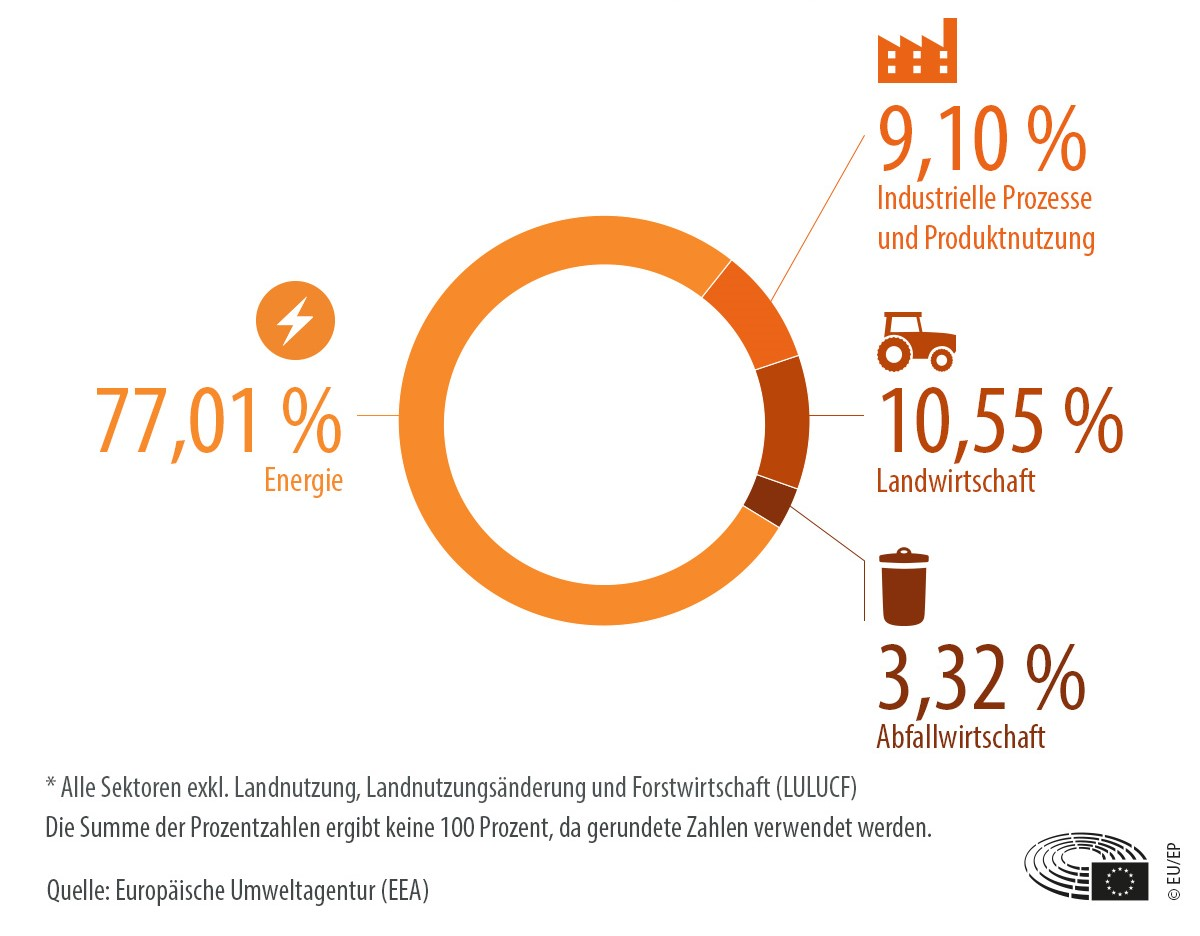
\includegraphics[height=6cm]{Bilder/em_sector.png} 
        		\end{center}
      	}%
        \newcommand{\slideOneTitle}{%
        		Treibhausgasemissionen in der EU nach Sektoren (2019)
       	}%
        	\newcommand{\slideTwo}{%
        		\vspace{-1cm}
            	\begin{center}
            	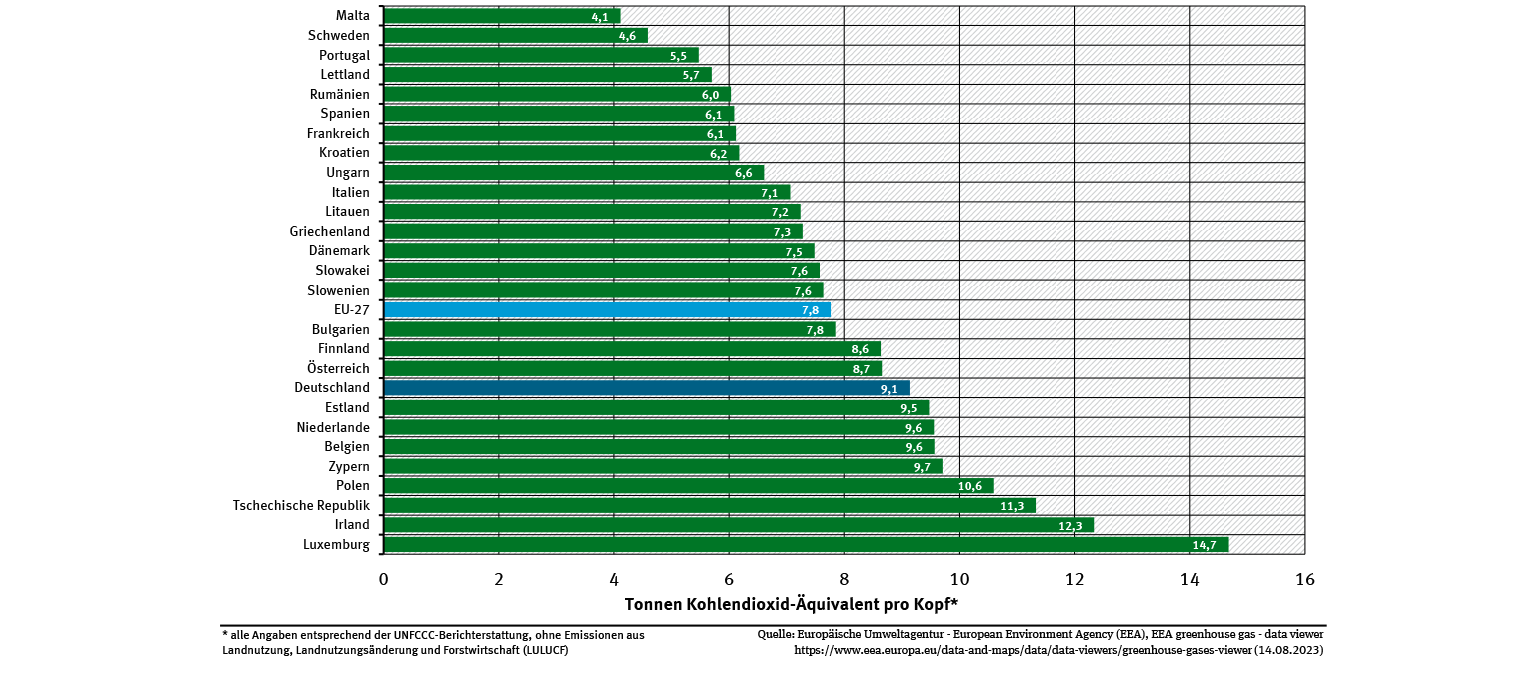
\includegraphics[height=6cm, width=\textwidth]{Bilder/em_vergleich.png}
            \end{center}
      	}%
        	\newcommand{\slideTwoTitle}{%
        		Pro-Kopf-Treibhausgas-Emissionen der Europäischen Union im Vergleich (2021)
       	}%
       	\newcommand{\slideThree}{%
        		\vspace{-1cm}
            	\begin{itemize}
            		\item 1992: Klimarahmenkonvention der Vereinten Nationen (UNFCCC)
	           	\item 1997: Erstes völkerrechtliches Abkommen mit bindenden Treibhausgas-Reduktionszielen (Kyoto Protokoll)
    		       	\item 2005: Einführung eines EU-weiten $CO_2$-Zertifikate-Handels
        		    	\item 2015: Pariser Abkommen
            		\begin{itemize}
            			\item Ziel: 1,5\degree C, maximal 2\degree C globale Erwärmung
                		\item Staaten setzen sich selbst verbindliche Ziele
	            	\end{itemize}
    		       	\item 2019: Europäischer Green Deal
	            	\begin{itemize}
    		        		\item Ziel: erster klimaneutraler Kontinent bis 2050
        		        	\item Viele Bereiche umfassendes Paket an Klimaschutzmaßnahmen
				\end{itemize}
    			\end{itemize}
  		}%
      	\newcommand{\slideThreeTitle}{%
        		Geschichte der internationalen und EU-Klimaschutzpolitik
       	}%
       	\newcommand{\slideFour}{%
        		\vspace{-1.25cm}
           	\begin{center}
			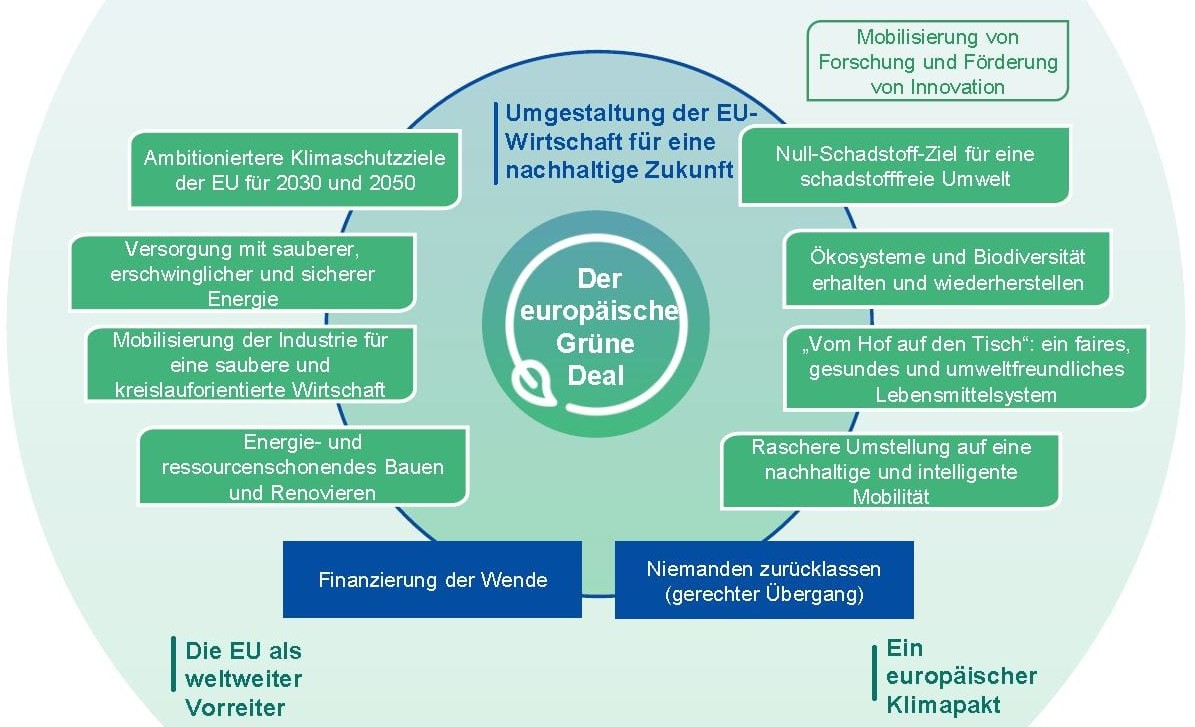
\includegraphics[height=6cm, width=\textwidth]{Bilder/green_deal.png}
            	\end{center}
      	}%
       	\newcommand{\slideFourTitle}{%
        		EU Green Deal
        }%
	}%
	{Migration}{
		\newcommand{\ausschuesse}{%
       		\begin{enumerate}
           		\item Ausschuss für bürgerliche Freiheiten, Justiz und Inneres (LIBE)
                	\item Ausschuss für Auswärtige Angelegenheiten (AFET)
                	\item Unterausschuss für Menschenrechte (DROI)
         	\end{enumerate}
      	}
       	\newcommand{\topic}{Asyl- und Migrationspolitik}
        \newcommand{\slideOne}{%
        		\vspace{-1cm}
			\begin{center}
        		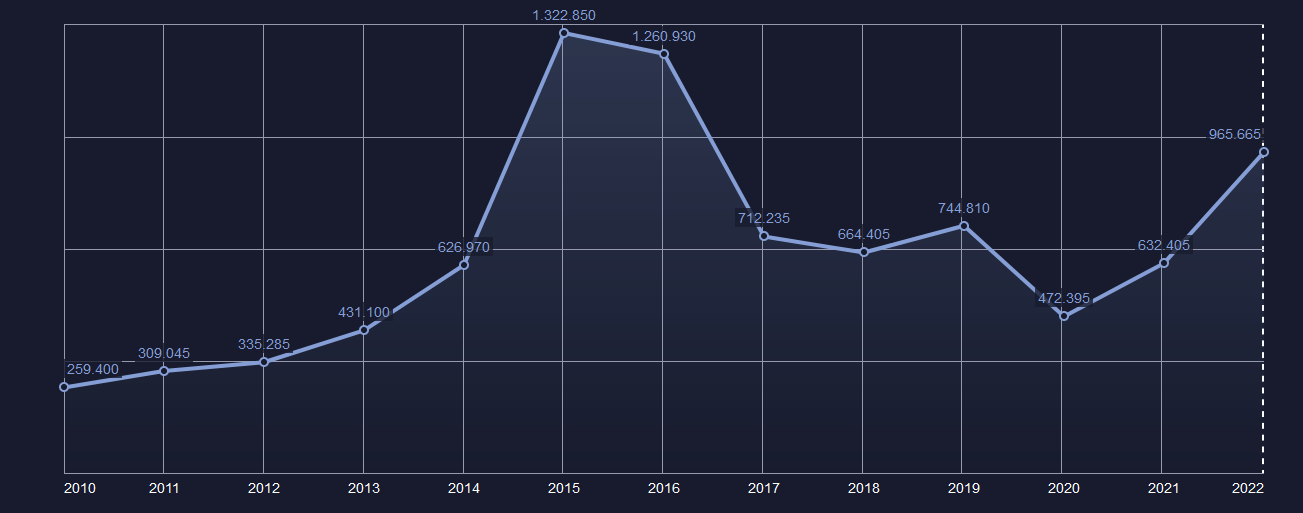
\includegraphics[height=6cm, width=\textwidth]{Bilder/asyl_num.png} 
        		\end{center}
      	}
        \newcommand{\slideOneTitle}{%
        		Entwicklung der Anzahl der Asylanträge \newline in der EU
      	}
      	\newcommand{\slideTwo}{%
        		\vspace{-1cm}
            	\begin{center}
            	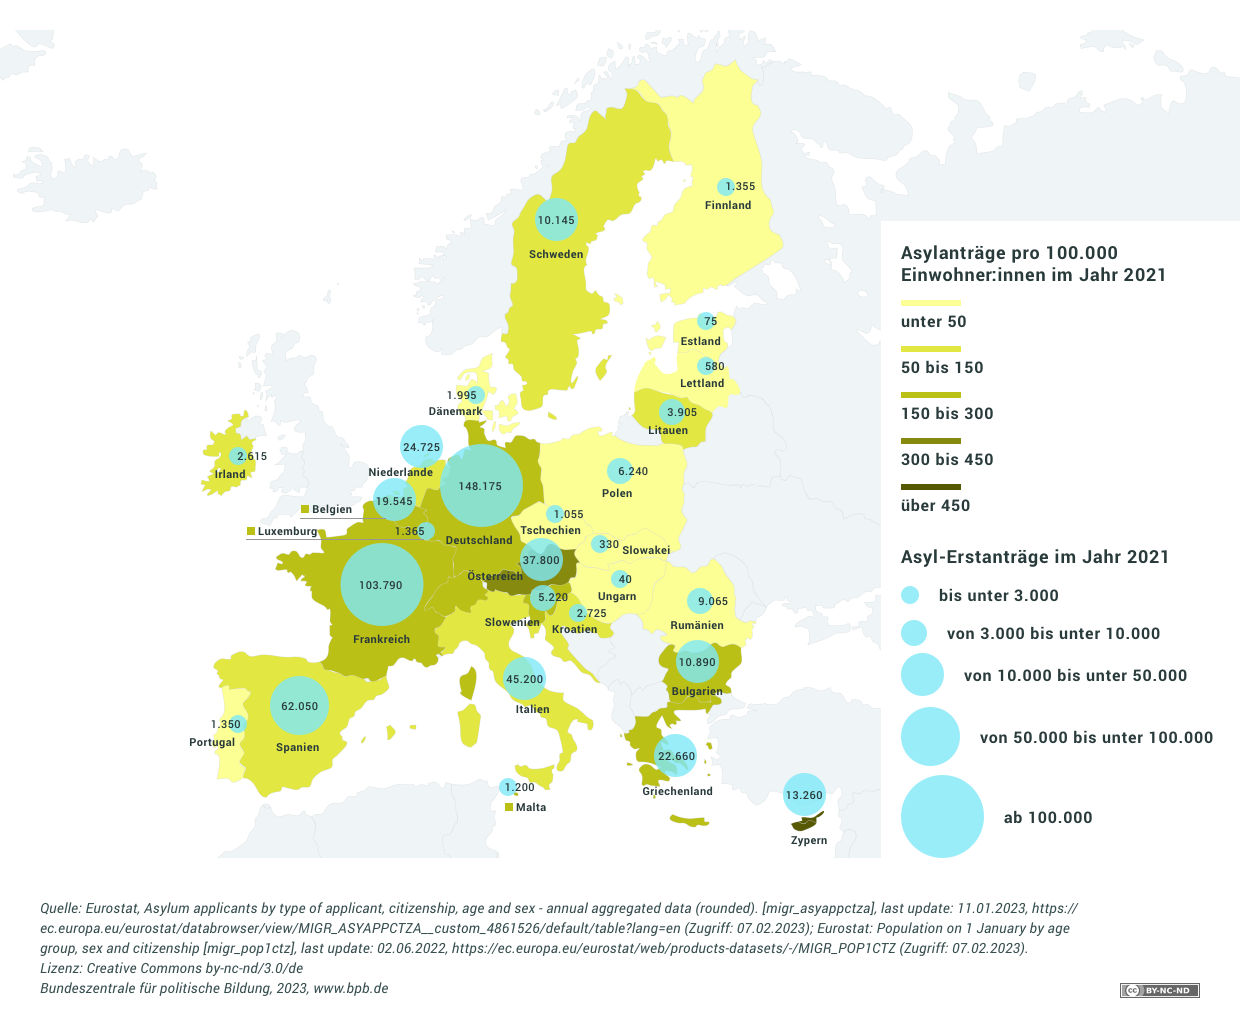
\includegraphics[height=6cm]{Bilder/asyl_capita.png} 
           	\end{center}
       	}
       	\newcommand{\slideTwoTitle}{%
        		Anzahl der Asyl-Anträge pro Mitgliedstaat (2021)
     	}
       	\newcommand{\slideThree}{%
        		\vspace{-1cm}
            	\begin{center}
            	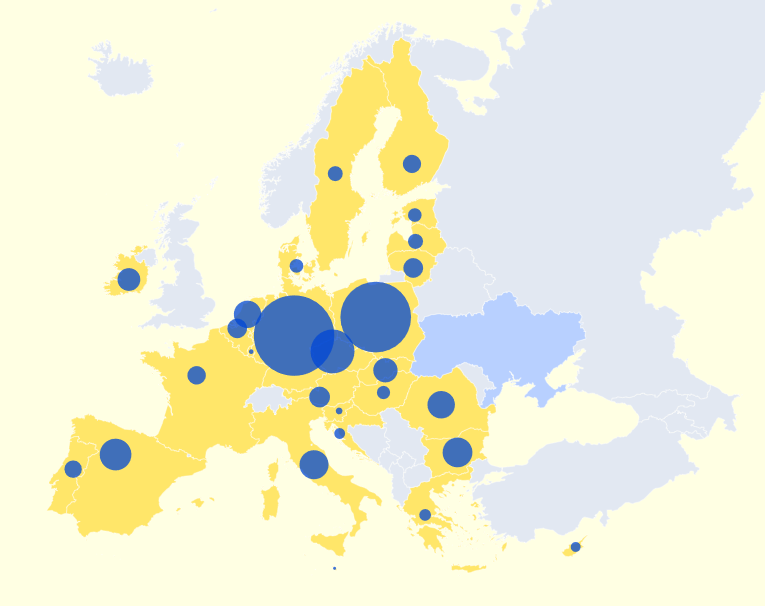
\includegraphics[height=6cm]{Bilder/ukraine.png} 
           	\end{center}
     	}
       	\newcommand{\slideThreeTitle}{%
        		Anzahl der aufgenommenen Geflüchteten aus der Ukraine (2023)
      	}
        	\newcommand{\slideFour}{%
      		\vspace{-1cm}
            	\begin{itemize}
            		\item 1997: Dublin Übereinkommen
                	\begin{itemize}
	                	\item Erste Vereinheitlichung der europäischen Asylpolitik
               		\item Zuständig für Asylsuchende ist Einreisestaat
                	\end{itemize}
    				\item 2004: Gründung Frontex (Grenz- und Küstenwache)
                	\item 2014: Einführung Asyl-, Migrations- und Integrationsfonds
                	\item 2023: EU-Asylkompromiss
                	\begin{itemize}
                		\item Asylverfahren an Außengrenze
                    	\item Solidaritätsmechanismus für Staaten mit Außengrenze (Aufnahme oder Ausgleichszahlungen)
               	\end{itemize}                
          	\end{itemize}
       	}
       	\newcommand{\slideFourTitle}{%
        		Geschichte der Europäischen Asyl- und Migrationspolitik
                }
		}%
	{Armee}{
		\newcommand{\ausschuesse}{%
     		\begin{enumerate}
            		\item Haushaltsausschuss (BUDG)
                	\item Ausschuss für bürgerliche Freiheiten, Justiz und Inneres (LIBE)
               	\item Unterausschuss für Sicherheit und Verteidigung (SEDE)
          	\end{enumerate}
       	}
        	\newcommand{\topic}{Außen- und Sicherheitspolitik}
       	\newcommand{\slideOne}{%
        		\vspace{-1cm}
            	\begin{center}
            	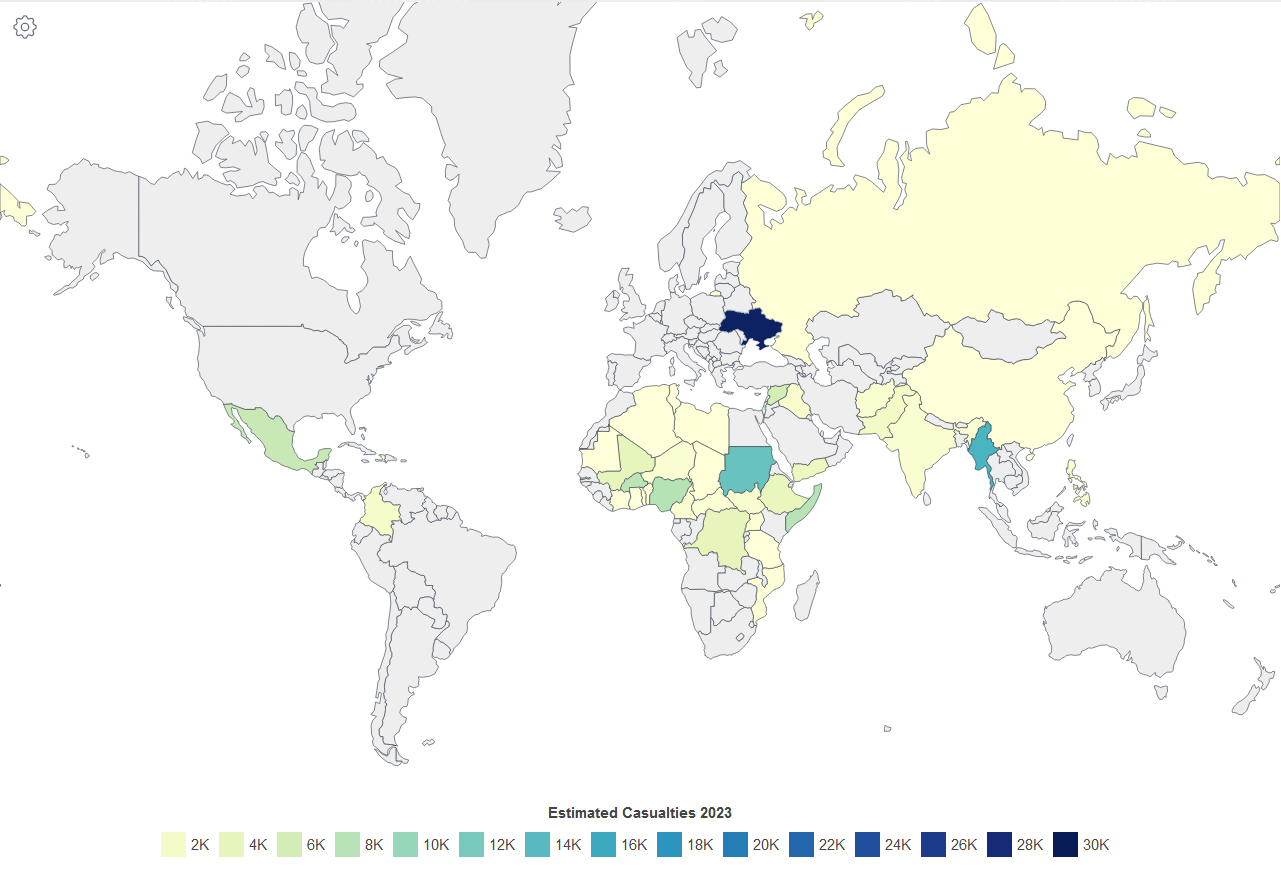
\includegraphics[height=6cm, width=\textwidth]{Bilder/conflicts.png} 
            	\end{center}
       	}
        	\newcommand{\slideOneTitle}{%
        		Todeszahlen in weltweiten Konflikten (2023)
        	}
        	\newcommand{\slideTwo}{%
        		\vspace{-1cm}
            	\begin{center}
            	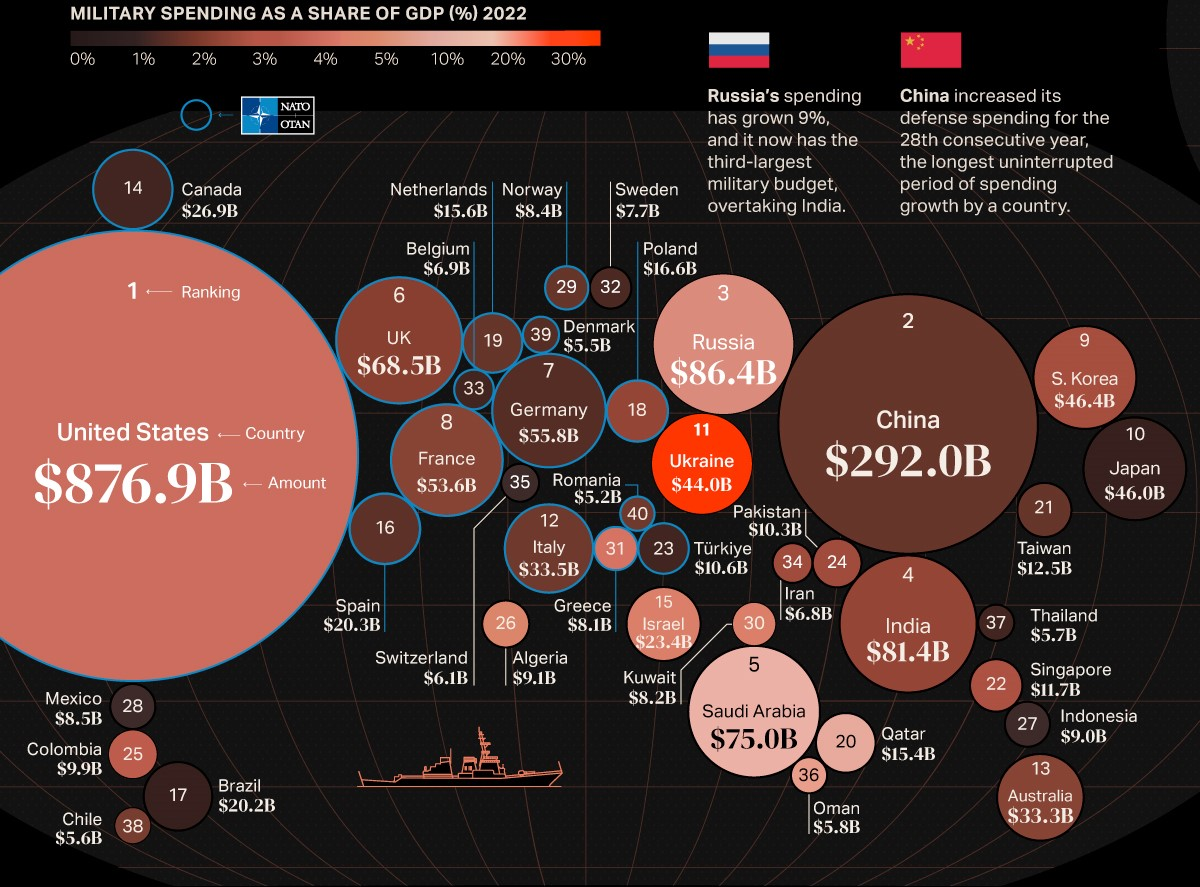
\includegraphics[height=6cm, width=\textwidth]{Bilder/mil_spend_world.png} 
            	\end{center}
      	}
        	\newcommand{\slideTwoTitle}{%
        		40 Länder mit höchsten Verteidigungsausgaben (2022)
       	}
        	\newcommand{\slideThree}{%
        		\vspace{-1cm}
            	\begin{center}
            	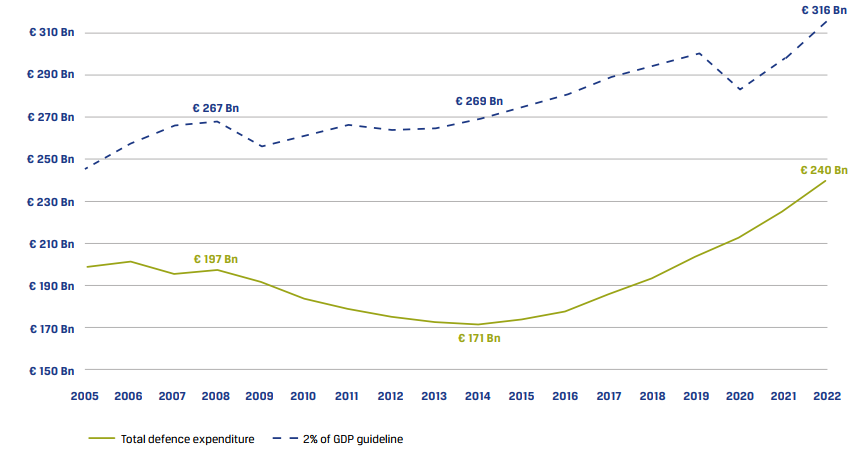
\includegraphics[height=6cm, width=\textwidth]{Bilder/mil_spend_eu.png} 
            	\end{center}
      	}
        	\newcommand{\slideThreeTitle}{%
        		Gesamte Verteidigungsausgaben der EU-Mitgliedstaaten (2005-2022)
       	}
       	\newcommand{\slideFour}{%
        		\vspace{-1cm}
            \begin{itemize}
            		\item 1954: Französische Nationalversammlung lehnt Europäische Armee ab, stattdessen Gründung Westeuropäische Union
              	\item 1992: Gemeinsame Außen- und Sicherheitspolitik (GASP)
             	\item 1999: Hoher Vertreter der EU für Außen- und Sicherheitspolitik
                	\item 2017: Vertiefte militärische Koordinierung durch Permanent Structured Cooperation (SSZ/PESCO)
          	\end{itemize}
        	}
        \newcommand{\slideFourTitle}{%
        		Geschichte der Europäischen Außen- und Sicherheitspolitik
       	}
	}%
}



%Information to be included in the title page:
\title{Simulation des Europäischen Parlaments}
\subtitle{Briefing}


\begin{document}
\frame{\titlepage}

\begin{frame}{Grußwort \politiker \newline (\politikerOffice)}
\vspace{-1cm}
    \begin{center}
        \includegraphics[height=4cm]{Bilder/Pol\_\city.png}
    \end{center}
\end{frame}

\begin{frame}{Die Jungen Europäischen Föderalist:innen (JEF)}
    \begin{minipage}[t]{0.7\textwidth}
    \vspace{-3.5cm}
        \begin{itemize}
            \item Proeuropäischer Jugendverband
            \item Überpartlich, überkonfessionell, unabhängig
            \item Sektionen in über 30 Ländern
            \item Ziel: Föderales Europa
            \item Kreisverband in \city
            \newline
            \item Was tun wir?
            \begin{itemize}
                \item Podiumsdiskussionen \& Infoveranstaltungen organisieren
                \item Europäischer Jugendaustausch
                \item Europapolitische Bildung
            \end{itemize}
        \end{itemize}
    \end{minipage}%
    \begin{minipage}[t]{0.25\textwidth}
        
\includegraphics[height=3.5cm]{Bilder/mitmachen.png}
    \end{minipage}
\end{frame}

\begin{frame}{Das Europäische Parlament}
\vspace{-1cm}
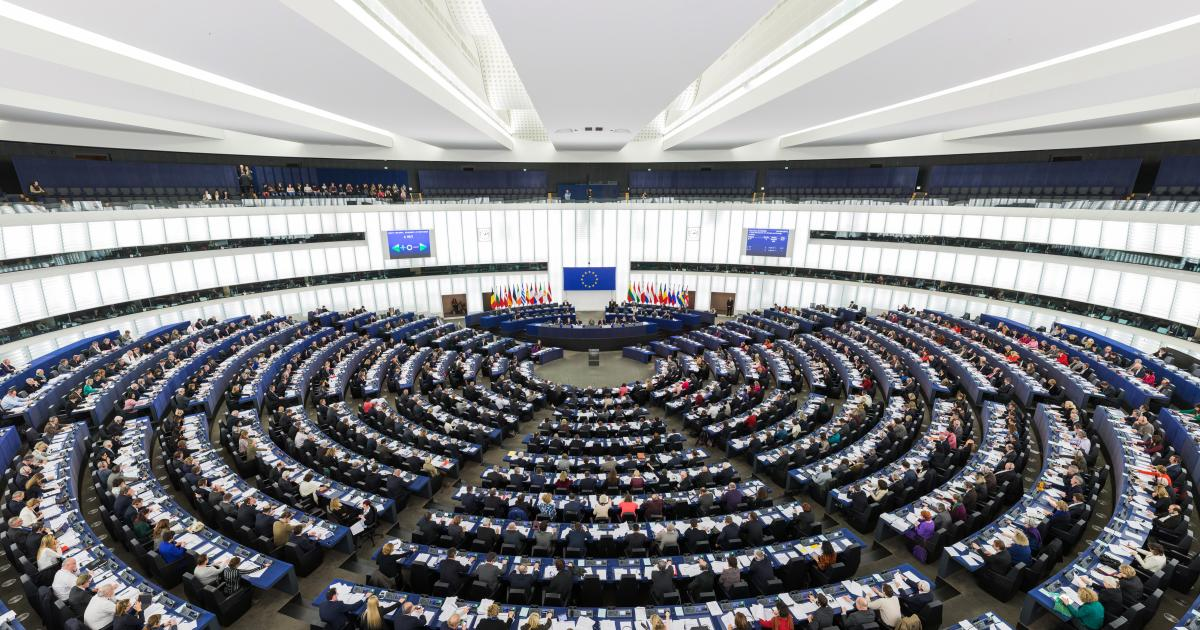
\includegraphics[width=\textwidth]{Bilder/ep.png}
\end{frame}

\begin{frame}{Das Europäische Parlament}
    \vspace{-0.5cm}
    \begin{itemize}
        \item 705 Abgeordnete (96 aus Deutschland)
        \item 27 Länder
        \item 7 Fraktionen
        \item Wahl alle 5 Jahre (9. Juni 2024)
    \end{itemize}
    \begin{center}
        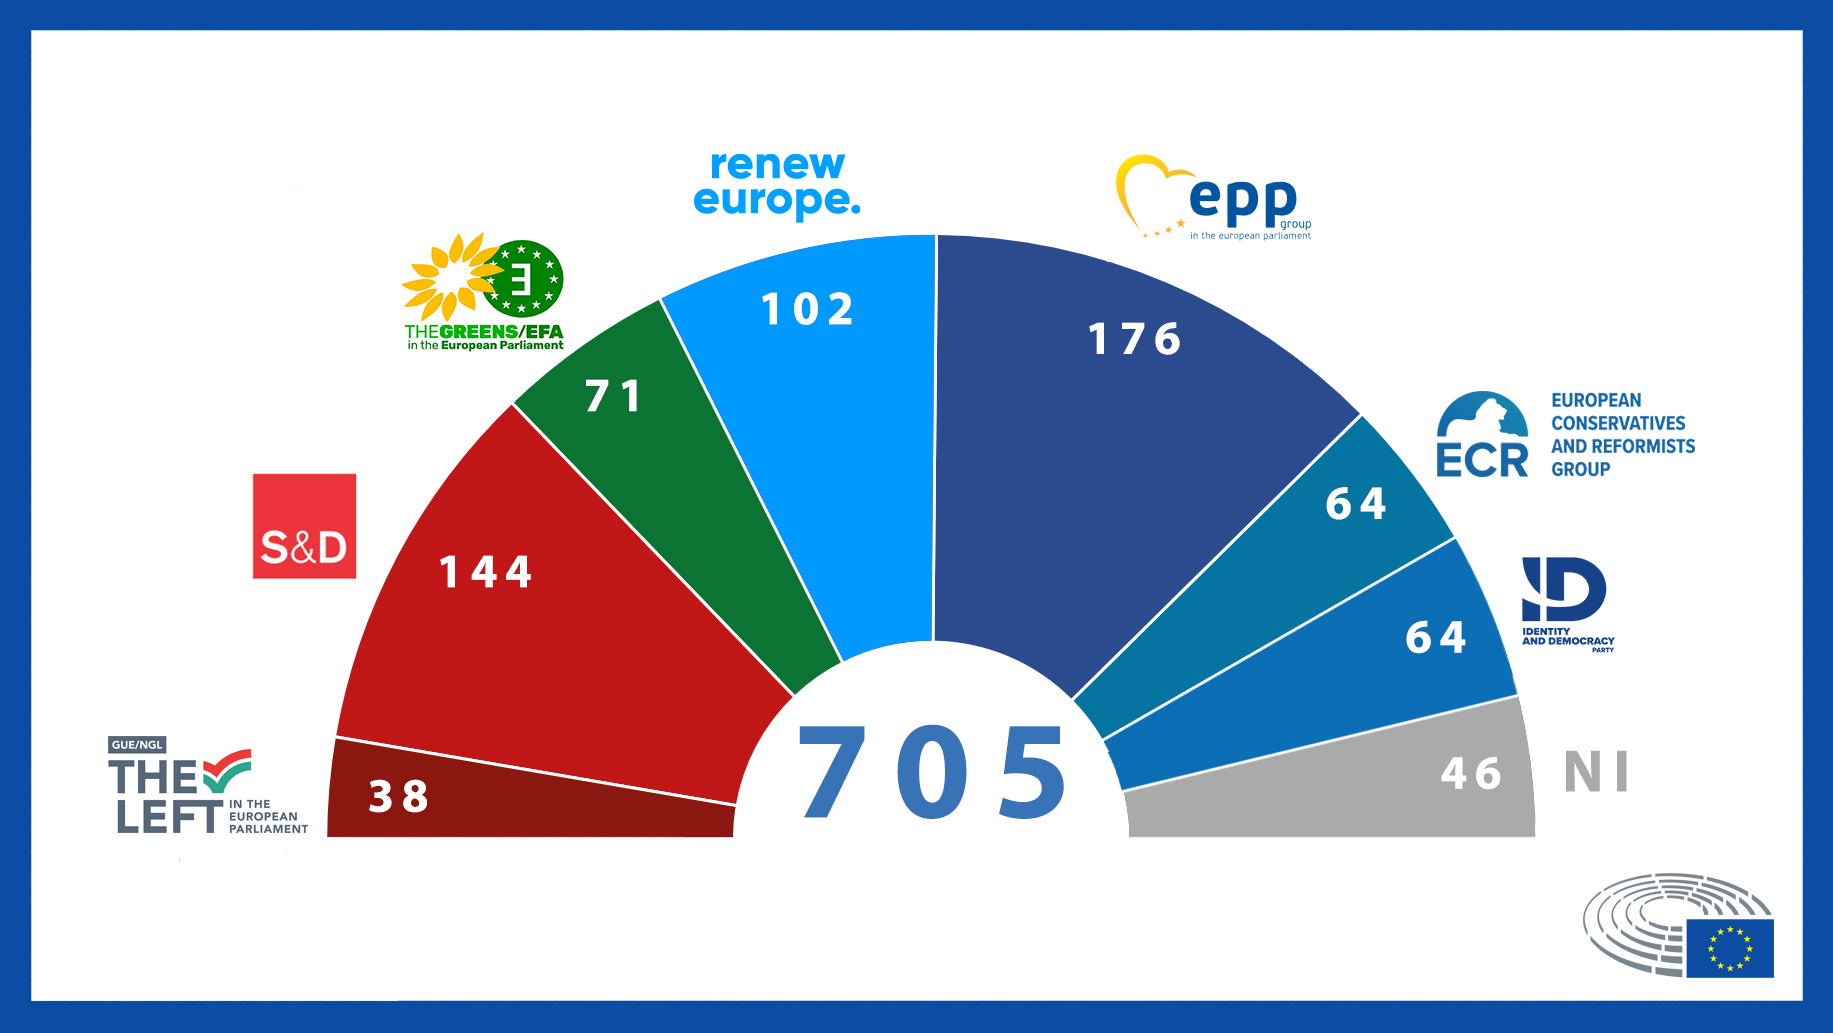
\includegraphics[height=3.5cm]{Bilder/EP_seats.jpg}
    \end{center}
\end{frame}

\begin{frame}{(Ordentliches) Gesetzgebungsverfahren in der EU}
\vspace{-0.5cm}
\begin{center}
    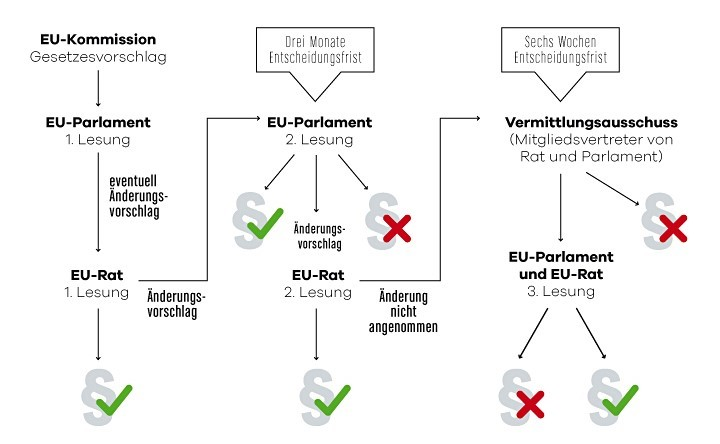
\includegraphics[height=6cm]{Bilder/gesetzgebungsprozess.jpg} 
\end{center}
\end{frame}

\begin{frame}{Involvierte Institutionen}
    \begin{figure}[!htb]
    \begin{minipage}[t]{0.32\textwidth}
        \begin{center}
        \vspace{-0.75cm}
        {\footnotesize \textbf{Europäische Kommission}}
        
        \begin{itemize}
            \item {\scriptsize erarbeitet Gesetzesvorschlag}
        \end{itemize} 
        \vspace{1.1cm}
        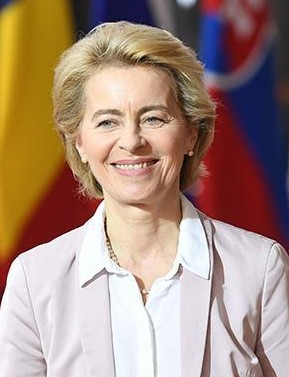
\includegraphics[height=2.5cm]{Bilder/vdl.png}
        \caption*{\tiny Ursula von der Leyen (EVP)}
        \end{center}
    \end{minipage}\hfill
    \begin{minipage}[t]{0.32\textwidth}
        \begin{center}
        \vspace{-0.75cm}
        {\footnotesize \textbf{Europäisches Parlament}}
        \newline
        \begin{itemize}
            \item {\scriptsize debattiert Vorschlag}
            \item {\scriptsize kann diesen ändern, annehmen oder ablehnen}
        \end{itemize}
        \vspace{0.1cm}
        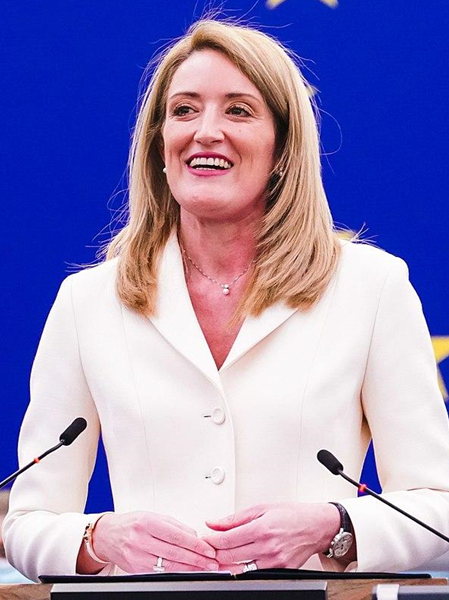
\includegraphics[height=2.5cm]{Bilder/metsola.png}
        \caption*{\tiny Roberta Metsola (EVP)}
        \end{center}
    \end{minipage}\hfill
    \begin{minipage}[t]{0.32\textwidth}
        \begin{center}
        \vspace{-0.75cm}
        {\footnotesize \textbf{Rat der EU}}
        \newline
        \begin{itemize}
            \item {\scriptsize debattiert Vorschlag}
            \item {\scriptsize kann diesen ändern, annehmen oder ablehnen}
        \end{itemize}
        \vspace{0.1cm}
        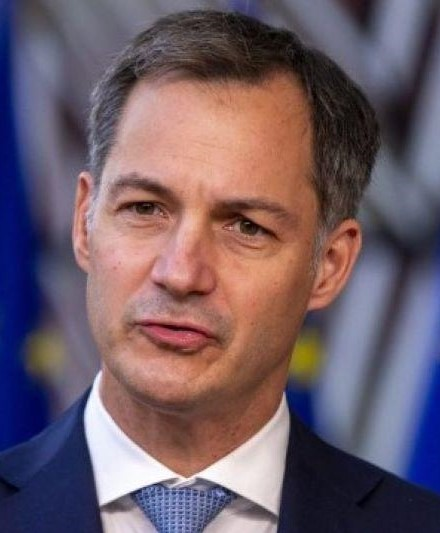
\includegraphics[height=2.5cm]{Bilder/decroo.png}
        \caption*{\tiny Alexander de Croo (Renew)}
        \end{center}
    \end{minipage}
    \end{figure}
\end{frame}


\begin{frame}{Arbeitsweise des Europäischen Parlaments}
    \vspace{-1cm}
    \begin{itemize}
        \item Hauptsächliche inhaltliche Arbeit in Ausschüssen
        \item Aktuell 20 Ausschüsse mit 25 bis 88 Abgeordneten
        \item Jeder Ausschuss beschäftigt sich mit einem bestimmten Sachbereich
        \item Relevante Ausschüsse für \topic:
        \ausschuesse
    \end{itemize}
\end{frame}

\begin{frame}{\slideOneTitle}
    \slideOne
\end{frame}

\begin{frame}{\slideTwoTitle}
    \slideTwo
\end{frame}

\begin{frame}{\slideThreeTitle}
    \slideThree
\end{frame}

\begin{frame}{\slideFourTitle}
    \slideFour
\end{frame}

\begin{frame}{Ablaufplan}
    \vspace{-1.5cm}
    \begin{itemize}
        \item \timeEinf: Einführung
        \item \timeFrakOne: 1. Fraktionssitzung
        \item \timeAuss: Ausschusssitzung
        \item \timeMittag: Mittagspause
        \item \timeFrakTwo: 2. Fraktionssitzung
        \item \timePlenar: Plenarsitzung
    \end{itemize}
\end{frame}

\begin{frame}{1. Fraktionssitzung}
    \begin{table}[h]
        \centering
        \begin{tabular}{c|c|c}
             Fraktion & Fraktionssaal & Fraktionsleitung \\
             \hline
             EVP & \evpRoom & \evpLeader \\
             S\&D & \sdRoom & \sdLeader \\
             Renew & \reRoom & \reLeader \\
             Grüne &\greenRoom & \greenLeader \\
             ID & \pfeRoom & \pfeLeader \\
        \end{tabular}
    \end{table}
\end{frame}

\end{document}